\documentclass[10pt,openany,a4paper]{article}
\usepackage{graphicx} 
\usepackage{multirow}
\usepackage{enumitem}
\usepackage{amssymb}
\usepackage{amsmath}
\usepackage{amsthm}
\usepackage{xcolor,color}
\usepackage{multicol}
\usepackage{multirow}
\usepackage{array}
\usepackage{animate}
\usepackage{amsthm}
\usepackage{caption}
\usepackage{minted}
\usepackage{fancyhdr}
\usepackage{geometry}
	\geometry{
		total = {160mm, 237mm},
		left = 30mm,
		right = 35mm,
		top = 35mm,
        bottom = 30mm,
        headheight=2cm
	}
\renewcommand{\headrulewidth}{0pt}

\graphicspath{{C:/Users/teoso/OneDrive/Documents/Tugas Kuliah/Template Math Depart/}}

\newcommand{\R}{\mathbb{R}}
\newcommand{\N}{\mathbb{N}}
\newcommand{\Z}{\mathbb{Z}}
\newcommand{\Q}{\mathbb{Q}}
\newcommand{\jawab}{\textbf{Solusi}:}

\pagestyle{fancy}
\fancyhf{}
\fancyhead[L]{
\includegraphics[width=1.6cm]{Provicom.png}}
\fancyhead[C]{\textbf{\MakeUppercase{Latihan Evaluasi Akhir Semester}\\ 
                \MakeUppercase{Semester Genap 2024/2025}\\ 
                \MakeUppercase{Departemen Matematika - FSAD ITS}\\ 
                \MakeUppercase{Program Sarjana}}}
\fancyhead[R]{\includegraphics[width=1.6cm]{provicomIG.png}}
\begin{document}
\indent
\textbf{Aturan Pengerjaan:}
\begin{itemize}
    \item Dilarang bekerja sama dalam bentuk apa pun. Segala jenis pelanggaran (mencontek, kerjasama, dsb) yang dilakukan saat EAS akan dikenakan sanksi pembatalan mata kuliah pada semester yang sedang berjalan.
    \item Tuliskan Pakta Integritas di awal lembar jawaban Anda, sebagai berikut: ``Dengan ini saya menyatakan bahwa saya mengerjakan sendiri tanpa bantuan dan membantu orang lain dalam menyelesaikan soal-soal EAS Alpro 2'' dan ditandatangani.
\end{itemize}

\noindent
Kerjakan dari yang termudah dulu yak !
\begin{enumerate}
    \item \textbf{(Skor: 25)}  
    Implementasikan konsep \textit{class} dan \textit{object}, \textit{constructor}, \textit{encapsulation}, dan \textit{inheritance} berikut.  
    Buat dua \texttt{class} dalam Java:
    \begin{itemize}
        \item \texttt{class Person} dengan atribut \texttt{name} (String) dan \texttt{age} (int). Buat \textit{constructor} penuh untuk menginisialisasi keduanya. Semua atribut bersifat \textit{private}, dan sediakan \textit{getter} serta \textit{setter} untuk masing-masing.
        \item \texttt{class Student} yang \textit{extends} \texttt{Person}. Tambahkan atribut \texttt{studentId} (String) dan \texttt{gpa} (double). Buat \textit{constructor} yang memanggil \textit{super(...)} untuk \texttt{name} dan \texttt{age}, kemudian menginisialisasi \texttt{studentId} dan \texttt{gpa}. Semua atribut \texttt{Student} juga \textit{private}, dengan \textit{getter} dan \textit{setter}.
    \end{itemize}
    \noindent
    Setelah itu, dalam metode \texttt{main}, buat satu objek \texttt{Student} dengan \texttt{name = "Budi"}, \texttt{age = 20}, \texttt{studentId = "S12345"}, \texttt{gpa = 3.75}. Tampilkan semua informasi \texttt{Student} tersebut (gunakan \texttt{System.out.println(...)}).
    
    \begin{minted}[fontsize=\footnotesize,frame=lines,framesep=2mm,linenos]{java}
// Lengkapi kode di bawah ini:

public class Person {
    private String name;
    private int age;

    // Constructor penuh
    public Person( ... ) {
        ...
    }

    // Getter dan Setter
    public String getName() { ... }
    public void setName(String name) { ... }
    public int getAge() { ... }
    public void setAge(int age) { ... }
}

public class Student extends Person {
    private String studentId;
    private double gpa;

    // Constructor
    public Student( ... ) {
        // Panggil super(...) di sini
        ...
    }

    // Getter dan Setter untuk studentId dan gpa
    public String getStudentId() { ... }
    public void setStudentId(String studentId) { ... }
    public double getGpa() { ... }
    public void setGpa(double gpa) { ... }
}

public class TestStudent {
    public static void main(String[] args) {
        // Buat objek Student dengan nama "Budi", age 20, studentId "S12345", gpa 3.75
        ...
        // Tampilkan semua informasi Student
        ...
    }
}
    \end{minted}

    \item \textbf{(Skor: 25)}  
    Perhatikan potongan kode di bawah, yang menggabungkan \textit{interface} dan \textit{abstract class}. Terdapat beberapa kesalahan (\textit{compile error}) terkait \textit{abstract method}, \textit{implementation}, dan \textit{return type}. Tugas Anda adalah menemukan dan memperbaiki kesalahan-kesalahan tersebut sehingga kode dapat dikompilasi dan dijalankan dengan benar.
    
    \begin{minted}[fontsize=\footnotesize,frame=lines,framesep=2mm,linenos]{java}
// Interface untuk entitas yang dapat menghitung volume
interface Volume {
    double calculateVolume(); // abstrak
}

// Abstract class untuk bangun ruang
abstract class Shape {
    protected String color;

    public Shape(String color) {
        this.color = color;
    }

    // Abstract method untuk menghitung luas permukaan
    public abstract double calculateSurfaceArea();

    // Method non-abstract mencetak informasi warna
    public void printColor() {
        System.out.println("Color: " + color);
    }
}

// Class Box yang harus meng-implement interface Volume dan menurunkan Shape
public class Box extends Shape implements Volume {
    private double length;
    private double width;
    private double height;

    // Constructor
    public Box(String color, double length, double width, double height) {
        // Panggil super constructor
        ...
        this.length = length;
        this.width = width;
        this.height = height;
    }
    
    // Lengkapi implementasi abstract method calculateSurfaceArea()
    public ... calculateSurfaceArea() {
        // Rumus: 2*(lw + lh + wh)
        return ...;
    }

    // Lengkapi implementasi interface calculateVolume()
    public ... calculateVolume() {
        // Rumus: length * width * height
        return ...;
    }

    // Tambahkan main untuk menguji:
    // Buat objek Box dengan color "Red", length 2.0, width 3.0, height 4.0,
    // Lalu panggil calculateSurfaceArea() dan calculateVolume(), serta printColor()
}
    \end{minted}

    \item \textbf{(Skor: 25)}  
    Berdasarkan spesifikasi berikut, buat \texttt{class} \texttt{Car}, kemudian buat satu \texttt{instance} dari \texttt{Car} di dalam \texttt{main}, dan tampilkan hasilnya:
    \begin{itemize}
        \item \texttt{Car} memiliki atribut \texttt{brand} (String), \texttt{model} (String), \texttt{year} (int), dan \texttt{mileage} (double). Semua atribut \textit{private}.
        \item Buat \textit{constructor} dengan parameter \texttt{brand}, \texttt{model}, \texttt{year}; \texttt{mileage} diinisialisasi default \texttt{0.0}.
        \item Buat \texttt{getter} untuk semua atribut, dan \texttt{setter} hanya untuk \texttt{mileage}.
        \item Buat method \texttt{drive(double km)} yang menambahkan nilai \texttt{mileage} dengan \texttt{km}.
        \item Buat method \texttt{toString()} yang mengembalikan \texttt{String} dengan format:  
        \texttt{"\{brand\} \{model\}, Year: \{year\}, Mileage: \{mileage\} km"}  
        (misal: ``Toyota Corolla, Year: 2020, Mileage: 15000.5 km'').
    \end{itemize}
    \noindent
    \textit{Contoh:}\\
    Buat sebuah objek \texttt{Car} dengan \texttt{brand = "Toyota"}, \texttt{model = "Corolla"}, \texttt{year = 2020}. Kemudian panggil \texttt{drive(15000.5)} dan cetak \texttt{toString()}, hasilnya harus menampilkan:  
    \texttt{Toyota Corolla, Year: 2020, Mileage: 15000.5 km}
    
    \begin{minted}[fontsize=\footnotesize,frame=lines,framesep=2mm,linenos]{java}
// Lengkapi kode di bawah ini:

public class Car {
    private String brand;
    private String model;
    private int year;
    private double mileage;

    // Constructor
    public Car( ... ) {
        ...
    }

    // Getter untuk semua atribut
    public String getBrand() { ... }
    public String getModel() { ... }
    public int getYear() { ... }
    public double getMileage() { ... }

    // Setter hanya untuk mileage
    public void setMileage( ... ) { ... }

    // Method drive untuk menambahkan mileage
    public void drive(double km) {
        ...
    }

    // Override toString()
    @Override
    public String toString() {
        ...
    }

    // Main untuk menguji
    public static void main(String[] args) {
        // Buat objek Car brand "Toyota", model "Corolla", year 2020
        Car myCar = new Car(...);
        // Panggil drive(15000.5)
        myCar.drive(15000.5);
        // Cetak hasil toString()
        System.out.println(myCar.toString());
    }
}
    \end{minted}

    \item \textbf{(Skor: 25)}  
    Analisis diagram UML berikut yang mencakup konsep OOP mulai dari \textit{inheritance}, \textit{abstract class}, hingga \textit{interface}. Jawablah pertanyaan di bawahnya.\vspace{2mm}


    % 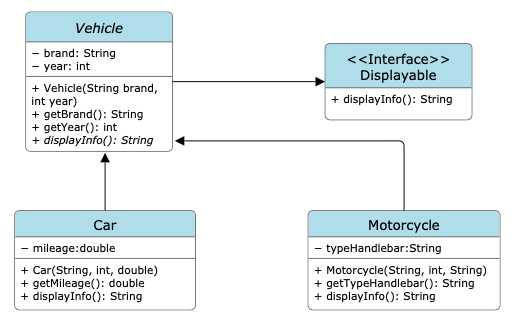
\includegraphics[width=12cm]{soal4.png}


    % \vspace{2mm}
    \begin{enumerate}[label=(\alph*)]
        \item Sebutkan tipe relasi antara \texttt{Vehicle}, \texttt{Car}, dan \texttt{Motorcycle}. Jelaskan singkat.\vspace{2mm}
        \item Mengapa \texttt{Vehicle} dideklarasikan sebagai \textit{abstract class} dan bukan \textit{interface}?\vspace{2mm}
        \item Tulis kode Java singkat untuk \texttt{class Car} yang mengimplementasikan semua metode yang diperlukan sesuai UML di atas. Sertakan \textit{keyword} yang tepat (\texttt{extends}, \texttt{implements}, \texttt{@Override}, dll.).\vspace{2mm}
        \item Bagaimana hubungan \texttt{Vehicle} dengan \texttt{Displayable}? Jelaskan bagaimana kelas-kelas di atas memenuhi kontrak \texttt{Displayable}.\vspace{2mm}
        \item Jika ingin menambahkan \texttt{class Truck} yang juga mewarisi \texttt{Vehicle} dan menambahkan atribut \texttt{loadCapacity} (double), bagaimana Anda menuliskan \textit{constructor} dan \textit{method} \texttt{displayInfo()} untuk \texttt{Truck}? Berikan contoh kode singkat.\vspace{2mm}
    \end{enumerate}
\end{enumerate}
\end{document}